\documentclass[letterpaper, 11pt]{article}

\usepackage{amsmath, amsthm, latexsym, amssymb, graphicx, bold-extra, mathrsfs, frcursive}
\usepackage[pdftex]{color}
\usepackage[T1]{fontenc}
\usepackage{listings}
\usepackage{adjustbox}
\usepackage{hyperref}
% Simplifies margin settings
\usepackage{geometry}
\geometry{margin=1in}

% Puts list item indicators in bold; makes flush with previous margin
\renewcommand\labelenumi{\bf\theenumi.}
\renewcommand\labelenumii{\bf\theenumii.}
% setlength\leftmargini{1.4em}
\setlength\leftmarginii{1.4em}

% Flexibility for headers and footers
\usepackage{fancyhdr}
\pagestyle{fancyplain}
\fancyhf{} %clear all header and footer fields
\lhead{\bf \small How To Write Fast Numerical Code \hspace*{\fill} Page \thepage}
\headsep 0.2in
\thispagestyle{empty}
\renewcommand{\headrulewidth}{0pt}
\renewcommand{\footrulewidth}{0pt}

\parindent 0in
\parskip 10pt
\setlength{\headheight}{20pt}

\title{ETH Zurich}

\begin{document}

%=======================================

\begin{center}
\Large \bf 263-2300-00: How To Write Fast Numerical Code

\Large \bf Assignment 3: 100 points

\large Submitted by Jinank Jain
\end{center}

\textbf{Solution 1}\\ \\
\textbf{Some technical details about test setup:}
\begin{itemize}
\item Compiler: clang-800.0.42.1
\item Machine: MacOSX Intel(R) Core(TM) i7-3520M CPU @ 2.90GHz
\item Processor Generation: Ivy Bridge
\item Flags: -O3 -fno-tree-vectorize -mavx -mavx2 -msse4.1
\end{itemize}
\begin{figure}[h!]
    \centering
    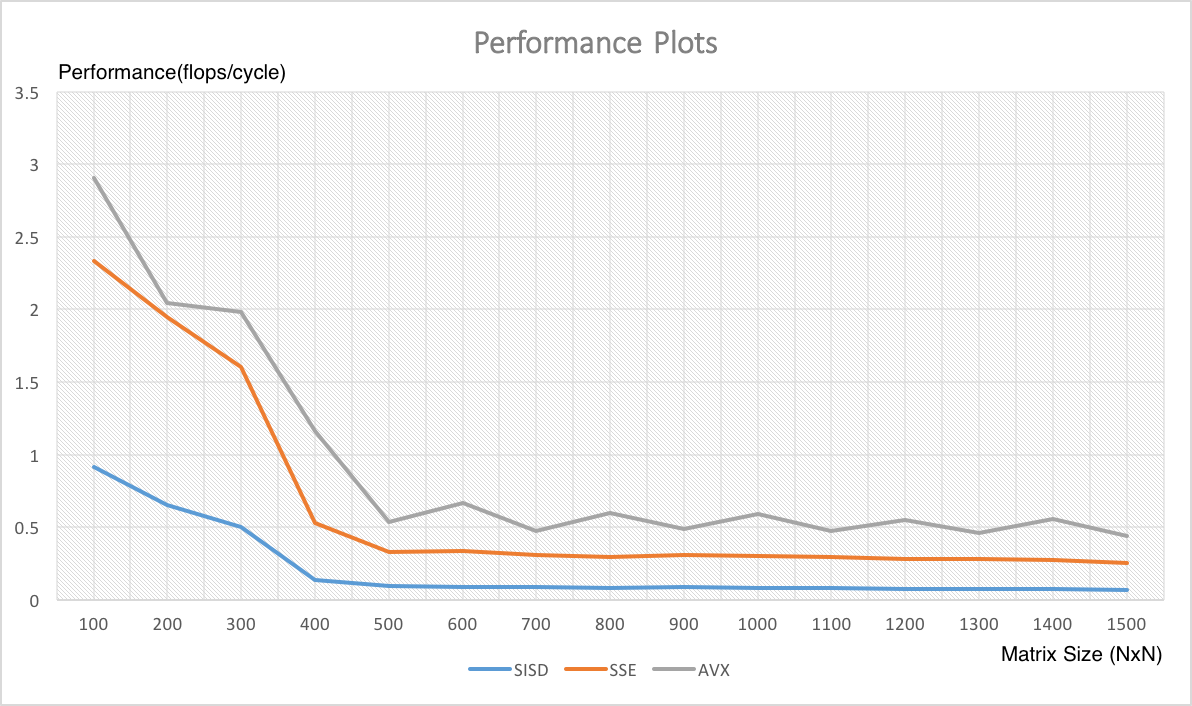
\includegraphics[width=100mm]{ques1}
    \caption{Plots for comparing SISD, SSE, and AVX implementation.}
    \label{fig:runtime}
\end{figure}
\begin{table}[]
\centering
\label{table1}
\begin{tabular}{|c|c|c|c|c|c|}
\hline
N    & SISD      & SSE      & AVX      & Speed Up (SSE/SISD) & Speed Up (AVX/SSE) \\ \hline
100  & 0.91 & 2.33 & 2.90 & 2.55         & 1.24        \\ \hline
200  & 0.65 & 1.94 & 2.04 & 2.97         & 1.05        \\ \hline
300  & 0.50 & 1.60 & 1.97 & 3.19         & 1.23        \\ \hline
400  & 0.13 & 0.52 & 1.16 & 3.84         & 2.20        \\ \hline
500  & 0.09 & 0.33 & 0.53 & 3.58         & 1.62        \\ \hline
600  & 0.08 & 0.33 & 0.66 & 3.81         & 1.99        \\ \hline
700  & 0.08 & 0.30 & 0.47 & 3.45         & 1.55        \\ \hline
800  & 0.07 & 0.29 & 0.59 & 3.74         & 2.03        \\ \hline
900  & 0.08 & 0.31 & 0.48 & 3.66         & 1.56        \\ \hline
1000 & 0.07 & 0.29 & 0.59 & 3.80         & 1.97        \\ \hline
1100 & 0.07 & 0.29 & 0.47 & 3.69         & 1.61        \\ \hline
1200 & 0.07 & 0.27 & 0.55 & 3.80         & 1.97        \\ \hline
1300 & 0.07 & 0.27 & 0.46 & 3.75         & 1.65        \\ \hline
1400 & 0.07 & 0.27 & 0.55 & 3.76         & 2.05        \\ \hline
1500 & 0.06 & 0.25 & 0.43 & 3.73         & 1.73        \\ \hline
\end{tabular}
\caption{Speed Up comparison between different implementation}
\end{table}
\textbf{Discussion about performance}\\
If we look at what happens when we move from SISD to SSE to AVX is basically instead of performing instruction on single double as in the case of SISD we perform instructions on 2 doubles and 4 doubles in case of AVX. So we look at it from the perspective of layman we should notice 2x and 4x speed up in the end. Other interesting aspect for this problem is looking at the Operational intensity for the problem is of the order $O(n)$ which means that the problem is compute bound so by vectorizing we should see more speed up as we can issue more instructions.
\bigskip

\textbf{Solution 2}\\ \\
\textbf{Some technical details about test setup:}
\begin{itemize}
\item Compiler: gcc version 4.8.5 20150623 (Red Hat 4.8.5-11) (GCC) 
\item Machine:  Intel(R) Core(TM) i7-6700 CPU @ 3.40GHz
\item Processor Generation: (Intel Skylake)
\end{itemize}
\textbf{Discussion about performance}\\
The main problem in this question is since the array size is not a multiple of 8(AVX vector size) we need to break the symmetry and do some sort mask loading in order to load a row from matrix A or vector x. Due to which problem size increases from 10x10 to 16x16 as we doing all those no ops and extra permutation to obtain the final answer which are usually expensive operation.

If we look from the layman prospective by vectorizing the code instead of performing single op we are able to perform 8 ops and we should see a performance increase of 8x but we are doing some futile computation by breaking the symmetry so we don't see perfect speed up in this case.
\bigskip

\textbf{Solution 3}\\ \\
\textbf{Some technical details about test setup:} 
\begin{itemize}
\item Compiler: clang-800.0.42.1
\item Machine: MacOSX Intel(R) Core(TM) i7-3520M CPU @ 2.90GHz
\item Processor Generation: Ivy Bridge
\end{itemize}
While running the experiments for benchmarking multiplication and division operations I ran each test 1000000 so that I can overcome all the noise which is there because of some variable initialization and some extra summation operation that I had to perform to fool the compiler. In order to determine the latency loop was designed in such a way that there was a dependency which would break the pipeling of multiple instructions and for getting throughput we need pipelling effect so in the loop I create a bunch(6) of instructions which would fill the pipeline always. Few more things which need to kept in mind while conducting experiments since I am repeating all the operations 1000000 times problems become numerically unstable so we should be wise enough to choose our operands. Operands selection could be found in code.

\textbf{Part a:} \\
Reference Values are taken from the manual provided before: \href{http://www.agner.org/optimize/instruction_tables.pdf}{Link} \\
If we look at the Table 2, I am almost able to reach the theoretical limit (Reference Value) in the Regular Case where I just multiply some bunch of random doubles or divide some numbers making sure that they stay in range and does not get eliminated as dead code by compiler. Main thing to note is result is pretty consistent with the theoretical values and which should be the case until and unless we are doing something really stupid. \\ \\
\textbf{Flags:} \texttt{ -O3 -fno-tree-vectorize -mno-sse4 -mno-sse3}
\leavevmode \newline
\begin{table}[h!]
\begin{adjustbox}{center}
\label{part3}
\begin{tabular}{|c|c|c|c|c|c|c|c|c|c|c|c|c|}
\hline
\textbf{Instruction} & \multicolumn{3}{c|}{\textbf{Reference Values}} & \multicolumn{3}{c|}{\textbf{Regular Case}} & \multicolumn{3}{c|}{\textbf{\begin{tabular}[c]{@{}c@{}}Special Case:\\ Mul: \\0x0000000000000001\end{tabular}}} & \multicolumn{3}{c|}{\textbf{\begin{tabular}[c]{@{}c@{}}Special Case:\\ Div: 2.0\end{tabular}}} \\ \hline
 & \textbf{Latency} & \textbf{TPS} & \textbf{Gap} & \textbf{Latency} & \textbf{TPS} & \textbf{Gap} & \textbf{Latency} & \textbf{TPS} & \textbf{Gap} & \textbf{Latency} & \textbf{TPS} & \textbf{Gap} \\ \hline
\textbf{MULSD} & 5 & 1 & 1 & 5.06 & 0.91 & 1.09 & 165.37 & 0.008  & 124.92 &NA  &NA  &NA  \\ \hline
\textbf{DIVSD} & 10-24 & .05-.12 & 8-18 & 20.06 & 0.07 & 14.06 &NA  &NA  &NA  &10.42  & 0.117  & 8.50  \\ \hline
\end{tabular}
\end{adjustbox}
\caption{Microbenchmarking for multiplication and division instruction}
\end{table}
\leavevmode \newline
\textbf{Flags:} \texttt{ -O3 -fno-tree-vectorize -mno-sse4 -mno-sse3 -ffast-math -funsafe-math-optimizations}
\begin{table}[h!]
\begin{adjustbox}{center}
\label{part3}
\begin{tabular}{|c|c|c|c|c|c|c|c|c|c|c|c|c|}
\hline
\textbf{Instruction} & \multicolumn{3}{c|}{\textbf{Reference Values}} & \multicolumn{3}{c|}{\textbf{Regular Case}} & \multicolumn{3}{c|}{\textbf{\begin{tabular}[c]{@{}c@{}}Special Case:\\ Mul: \\0x0000000000000001\end{tabular}}} & \multicolumn{3}{c|}{\textbf{\begin{tabular}[c]{@{}c@{}}Special Case:\\ Div: 2.0\end{tabular}}} \\ \hline
 & \textbf{Latency} & \textbf{TPS} & \textbf{Gap} & \textbf{Latency} & \textbf{TPS} & \textbf{Gap} & \textbf{Latency} & \textbf{TPS} & \textbf{Gap} & \textbf{Latency} & \textbf{TPS} & \textbf{Gap} \\ \hline
\textbf{MULSD} & 5 & 1 & 1 & 5.13 & 1.31 & 0.76 & 135.15 & 0.008  & 116.87 & NA  & NA  & NA  \\ \hline
\textbf{DIVSD} & 10-24 & .05-.12 & 8-18 & 19.02 & 0.38 & 2.63 &NA  &NA  &NA  &10.27  & 0.54  & 1.86  \\ \hline
\end{tabular}
\end{adjustbox}
\caption{Microbenchmarking for multiplication and division instruction}
\end{table}

\textbf{Part b:} \\
In this case we are working with denormal values like 0x0000000000000001 which are very small. Hence the production of a denormal number is sometimes called gradual underflow because it allows a calculation to lose precision slowly when the result is small. Handling denormal values in software always leads to a significant decrease in performance. In extreme cases, instructions involving denormal operands may run as much as 100 times slower and that is what we are experience in our case too. Gap and Latency becomes unpredicted and increase by almost a factor 30.
\\ \\ \\
\textbf{Part c:} \\
When we use 2.0 as a special division operand we need to keep in mind that our numerator is big enough for repeating the experiment 1000000 so that it does not become 0 and we do an no-op. For that I choose my numerator as 1e200 which is big enough for such computations. But the point to note is we are hitting the lower bound of latency which shows that there is some sort of optimizations that can be performed for operands like 2.0.

\textbf{Part d:} \\
In this case when we turn on mathematical optimizations \texttt{-ffast-math -funsafe-math-optimizations} we see some interesting stuff. If we look at gcc manual. The gcc manual says that this option "allows optimizations for floating-point arithmetic that (a) assume that arguments and results are valid and (b) may violate IEEE or ANSI standards."
Essentially, what this means is that the compiler will take certain shortcuts in calculating the results of floating-point operations, which may result in rounding errors or potentially the program?s malfunctioning (hence the unsafe part of the name).Therefore throughput and latency of double precision divisions are reduced to values similar to  floating point multiplications. Reason
is that compiler replaces all division instructions with appropriate multiplication values, and therefore
reduces total throughput and latency with cost of reduced precision.
\bigskip

\clearpage

%=======================================

\end{document}